\documentclass[10pt]{article}   	 
\usepackage{geometry}                		 
\geometry{a4paper}  
 
%\usepackage{draftwatermark}
%\SetWatermarkAngle{45}
%\SetWatermarkLightness{0.8}
%\SetWatermarkFontSize{4cm}
%\SetWatermarkScale{2}
%\SetWatermarkText{DRAFT  - NO DISTRIBUTION }
               		
\usepackage{graphicx}				
\usepackage{amssymb}
\usepackage{longtable}
\usepackage{listings} \lstset{numbers=left, numberstyle=\tiny, numbersep=5pt} \lstset{language=C}
\newcommand{\zwave}{Z-Wave \raise0.8ex\hbox{\tiny TM} }
\title{Z-Way Users Documentation}
\author{(c) Z-Wave.Me Team, based on Version 1.4}
\date{}							 

\begin{document}
\maketitle
\tableofcontents

\section {User Interfaces Intro}

The term Z-Way refers to a software architecture for a Z-Wave Network Controller that consists of several parts.

\begin{itemize}

\item {\bf The Z-Way server:} This software runs on top of your operating system or inside your appliance. It handles
all Z-Wave network related functions and has a built-in web server to support User Interfaces
\item {\bf The Demo User Interface:} This is one of the User Interfaces. It is not optimized in terms of design and fashion but
it will show all functions of the Z-Wave network and the Z-Wave devices and give users access to all data 
related to the management of a Z-Wave network and to the operation of Z-Wave devices in this network.
\item {\bf Other User Interfaces:} Z-Way provides several other user interfaces that offer a subset of the Demo User 
Interfaces functionality but may enhance them with own logic.
\end{itemize}

The next chapters describe the purpose and the use of the Z-Way server and the Demo User Interface. This means
that the following four areas are \underline{not scope of this manual}:

\begin{itemize}
\item {\bf Z-Way development:} There is a separate manual {\bf Z-Way Developers Manual} with instructions how to 
develop your own User Interface using the Z-Way Server. You can download this manual e.g. from the Z-Wave.Me 
Home Page www.z-wave.me.
\item {\bf Z-Wave Device Specific Information:} Each Z-Wave device has its own manual that may be needed for the 
the management and use of this device. For European products you can find a good collection of manuals
at http://manuals.zwaveeurope.com.
\item {\bf Z-Wave Basics:} Please refer to the book "Z-Wave basics" by Dr. Christian Paetz (paper back, 264 pages, 
ISBN 978-1490537368), for more information 
about Z-Wave in general and how the different functional levels of Z-Wave are designed and work. 
The book is available at various sources among them at Amazon. In case your local amazon store is not selling english 
books on default, please check the english book section for the book.

\item {\bf Other User Interfaces:} This manual will only briefly mention other user interfaces than the demo 
user interface below.
\end{itemize}

\subsection{iPhone / iPad Interface}

In todays world accessing the smart home from a mobile is a key feature. Z-Way provides a very basic but 
fully functional iPhone App in Objective C for download at GitHub \footnote{https://github.com/PoltoS/Z-Way-iOS}. 
You can also download the compiled version of the App from the Apple App Store - search for Z-Way.

\begin{figure} 
\begin{center}
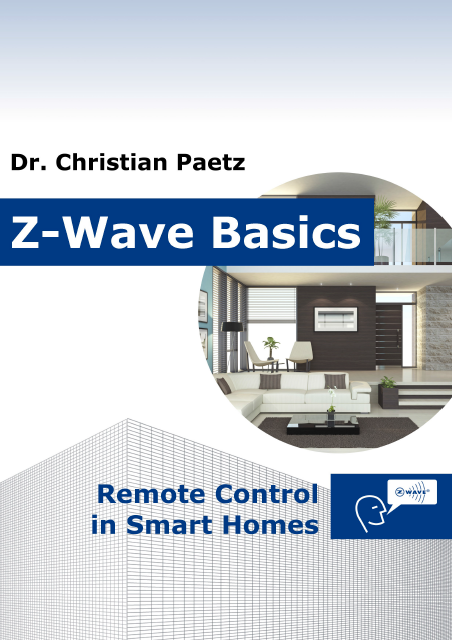
\includegraphics[scale=0.3]{pics/book.png}
\caption{Dr. Christian Paetz: Z-Wave Basics}
\label{c2:demorouting} 
\end{center} 
\end{figure}

\begin{figure} 
\begin{center}
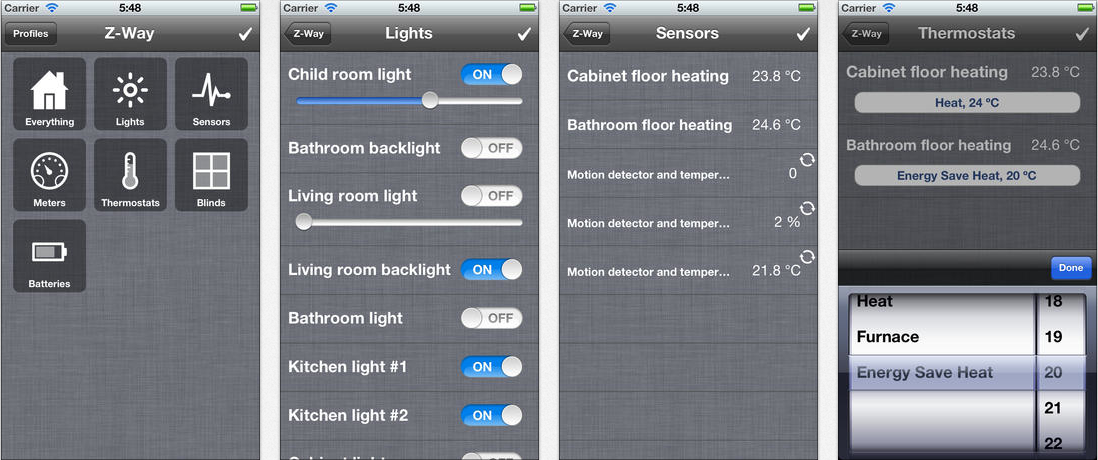
\includegraphics[scale=0.3]{pics/ipad.png}
\caption{iPhone/iPad App for Z-Way}
\label{c2:demorouting} 
\end{center} 
\end{figure}

\subsection{Mini Web UI}

The Mini UI Limited to about 800 lines of code this AJAX interface is a condensed version of the blue UI. 
It is a good starting point for writing AJAX based User Interfaces for RaZberry. You can download the most 
recent version of the mini UI free of charge from Github \footnote {https://github.com/PoltoS/z-way-mini-ui/}.

  
\section {Z-Wave Network Quick Basics}

\subsection{Network and controllers}

A Z-Wave network consists of various devices interconnected by a wireless communication protocol. Thanks to the 
Z-Wave standard products from different vendors can work together seamlessly. 

Another advantage of Z-Wave is their ability to act as repeaters and forward data packets between nodes 
not able to communicate directly over the air. This extends the range of a Z-Wave network and improves 
stability. In order to perform this packet routing and forwarding the particular node needs to be mains 
powered. Battery operated nodes can’t act as repeaters.

Z-Wave differentiates between portable and static controllers to control other devices. Portable 
controllers change their location and they are battery powered. To allow long battery life-time 
they are inactive most of the time and will only communicate with other devices during manual 
interaction (pressing a button). 

Static controllers are installed on a fixed location. They are mains powered and therefore able to 
stay alive all the time to communicate with other devices. 

Z-way implements a static controller and will usually be the primary controller handling all inclusions 
and exclusions of devices in and from the network.  However Z-Way can also be included as a secondary 
controller in other networks controlled by other Z-Wave controllers. Z-way will then follow the network 
setup of this other network.


\subsection{Inclusion and Configuration of various device types}

Z-Wave devices can be mains powered or battery operated.  The inclusion process for both devices types is 
similar, however battery operated devices need special handling.

\subsubsection{Mains Powered Devices}

A mains powered device is easy to configure after inclusion since the device will receive all configuration 
commands and execute them immediately. Mains powered devices are always listening to other commands and can 
repeat commands to other nodes. 

\subsubsection{Battery Operated Devices}

The main objective of a battery-operated device is to preserve the battery power and only use as much 
battery power as needed.  Battery powered devices are therefore in a deep-sleep state most of the time.
 In deep-sleep state they are not able to communicate with other devices. 

In order to communicate with an other device the battery-operated device needs to be woken up and send to 
sleep mode right after the communication took place. To maintain a minimal level of “responsiveness” and 
to allow to configure and to use battery-operated devices Z-Wave offers three basic solutions:
\begin{itemize}
\item Devices with wakeup intervals
\item Frequently listening battery devices 
\item Devices with manual wakeup
\end{itemize}

\subsubsection{Wakeup Interval}

Devices with wakeup interval will wakeup after a defined interval and send out a wakeup notification. 
Other devices such as the Z-Way controller are able to communicate with this device and send out messages 
to this device (The controller know about the status of the battery operated device and will queue messages 
in a waiting queue.) After all communication is done the controller is supposed to send the device back into 
deep sleep.
If no communication happens the battery-operated device will go back into deep sleep mode after a defined 
time (typically some seconds – up to one minute).

The best practice of Z-Wave suggests that battery operated devices stay awake for a defined time right 
after inclusion and go into deep sleep mode afterwards. This first awake-time is device dependent and 
varies from 1 minute to one hour.

Hence it is recommended to configure the device right after inclusion to make sure the device is still 
alive. If the battery operated device is already in sleep state all configuration commands will be 
queued and executed after the next scheduled wakeup if and only if a valid wakeup interval was configured 
during the first part of the configuration process. If this was not the case the device needs to be woken 
up manually.

If the device went already into deep sleep before the configuration was finished it is recommended to 
wake up the device manually to speed up the configuration process. Otherwise the configuration will happen 
after the next scheduled wakeup.

Some battery-operated devices may not go into sleep mode at all after inclusion but need to be sent into 
deep sleep after configuration is finished. This is done by Z-Way automatically.

The configuration of the wakeup interval is a tradeoff between maximum battery life-time  (suggest a 
very long wakeup interval with few wakeup cycles) and some responsiveness of the device in case of a 
network-reorganization. Typical values are between 5 minutes and 5 hours.

\subsubsection{Frequently Listening Devices}

Z-Wave has introduced frequently listening devices (FLIRS). These devices will wakeup at least once in 
a second and try to receive a message. The trick is that the wakeup is so short, that on average the power 
consumption of FLIRS devices are low enough to allow battery life times greater than one year. FLIRS 
devices can be configured without any problems like mains powered devices since every command will 
always be received latest after one second.
However FLIRS device will not route other devices messages to preserve battery power.

\subsubsection{Devices with manual wakeup}

Remote controls are battery operated as well but they are only awake if a button is pressed. Remote 
controls will not wakeup regularly to check for queued messages. Hence whenever a remote control is 
configured from the Z-Way controller, the device needs to be woken up manually. Please refer to the 
manual of the remote control for further instructions how to wakeup the device.  


  
\section{Z-Way Demo UI Basics}

The Z-Way Demo Web Interface can be used in two different modes:

\begin{itemize}
\item Simple Mode: All usage and basic administration functions are visible for inclusion, 
exclusion and configuration of the network. 

\item Experts Mode: The expert Mode offers additional interaction for fine-tuning the Z-Wave network
and to access internal data of Z-Way. This is particularly useful for developing own User Interface.
\end{itemize}
 
\begin{figure} 
\begin{center}
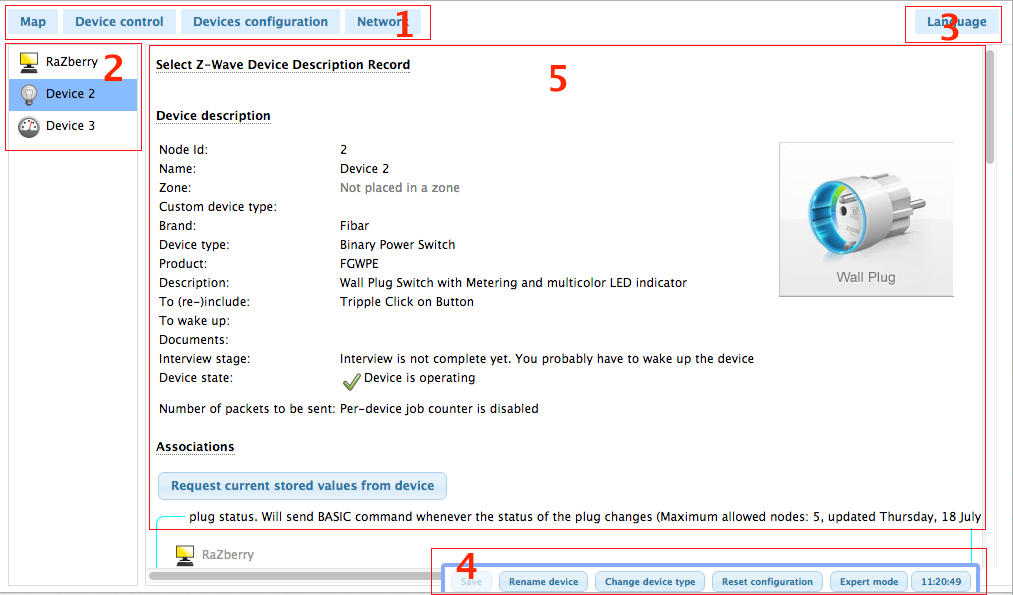
\includegraphics[scale=0.4]{pics/map3.png}
\caption{Sections of the Screen Estate}
\label{uc3:general} 
\end{center} 
\end{figure}


The total screen estate can be divided into different sections: 
\begin {enumerate}
\item {\bf The function Tabs:} Clicking on the function tabs leads to the different functions of Z-Way.
\item {\bf Left hand side:} Here you either find a list of devices, zones etc. Clicking on these icons opens a 
dialog on the dialog pane.
\item {\bf Language Selector:} Here you can pick a UI language of choice. Make sure to reload the page after changing
the language.
\item {\bf Bottom Context Menu:} The bottom context menu contains functions, which usually apply to all devices 
within the selected function tab.
\item {\bf Main Window:} This area context the main user dialog.
 
\end {enumerate}


\section{The Initial Setup} 

The initial setup is done one time only. But all settings can be changed later on.

Go to tab 'Map'. Here you can setup your zones (rooms) in your home by creating 
subzones of the root zone 'All'.  

\subsection{Load your own floor plan}

As first step you should replace the default zone map with your own floor plan. However you will be able to 
use Z-Way with the default floor plan as well.

Click the Button 'Upload Image' on the bottom line context menu and choose the new image from your local 
computer. You may upload image in the following file formats: JPG, PNG, GIF.

All changes will be saved after hitting the save button in the bottom context menu. Make sure to save 
all your changes!

\subsection{Define your zones/rooms}

Define all your rooms using the right click context menu on the left hands side tree. You can organize 
your rooms in a hierarchy or you can place all of them under the zone called 'All'.

Whenever you enter a new child zone into the tree you are required to mark the zone (room) in the floor 
plan on the right hand side. Just click into the right hand floor plan and mark the corners of the zone. 
Once you have completed the outer border you can drag the points you just placed. You can also move the 
whole zone object when click 
and hold into the middle of the object. Use the 'Enter' key to stop editing and escape to cancel. To save 
zone without drawing area click enter 
immediately after entering edit mode. Hold shift to draw straight lines. Stop this mode by clicking on 
'Stop Editing Zone' on the bottom end context menu.  For each individual child zone a new floor map can 
be uploaded. This allows for instance to have one 
overall map and certain sub parts or to have one map for each floor of the home.

Devices can be placed on each level of the floor plan hierarchy. The internally recognized place of 
the device is supposed to be the “deepest” child level zone.

\underline{Make sure to save your changes using the 'Save' button in the bottom context menu!}

\subsection{Place your devices}

\begin{figure} 
\begin{center}
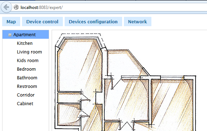
\includegraphics[scale=1.0]{pics/map2.png}
\caption{Floor Map}
 
\end{center} 
\end{figure}

If you have already included devices you can place them into the floor plan. Otherwise skip this step for the moment!

To place devices into the map activate the device list by clicking  'Place Devices' on the bottom 
context menu. A list of all available and not placed devices will appear on the left hand side below 
the zone tree. Just drag and drop the device icons into the floor plan. The devices will be assigned 
to the zone selected in the zone tree regardless of the place in the map. So it is possible to have 
a device assigned to a zone but not placed into the marked area of this zone.

When finished just click 'Stop Placing Devices'. All changes will be saved after hitting the save 
button in the bottom context menu. Make sure to save all your changes!

\subsection{Name your devices}

Once devices are placed on the map they can be renamed. Just click  'Show devices in tree' in the 
bottom context menu to show all devices in their respective zones. Right clicking on the Device 
default name ('Device' plus Node Id) opens a dialog to change the name.

\underline{Make sure to save your changes using the 'Save' button in the bottom context menu!}

\begin{quote} {\bf 

For every device included into Z-Way the following steps need to be done.
\begin{enumerate}
\item In the tab “Network Management” include the device into the network. 
\item Check in Device Status Tab if the interview was completed.
\item In the tab “Device Configuration” configure device specific parameters. 
\item In the tab “Zones” place the devices in the area they belong to and rename it. 
\end{enumerate}
}
\end{quote}


\section{Network Management}

 
\begin{figure} 
\begin{center}
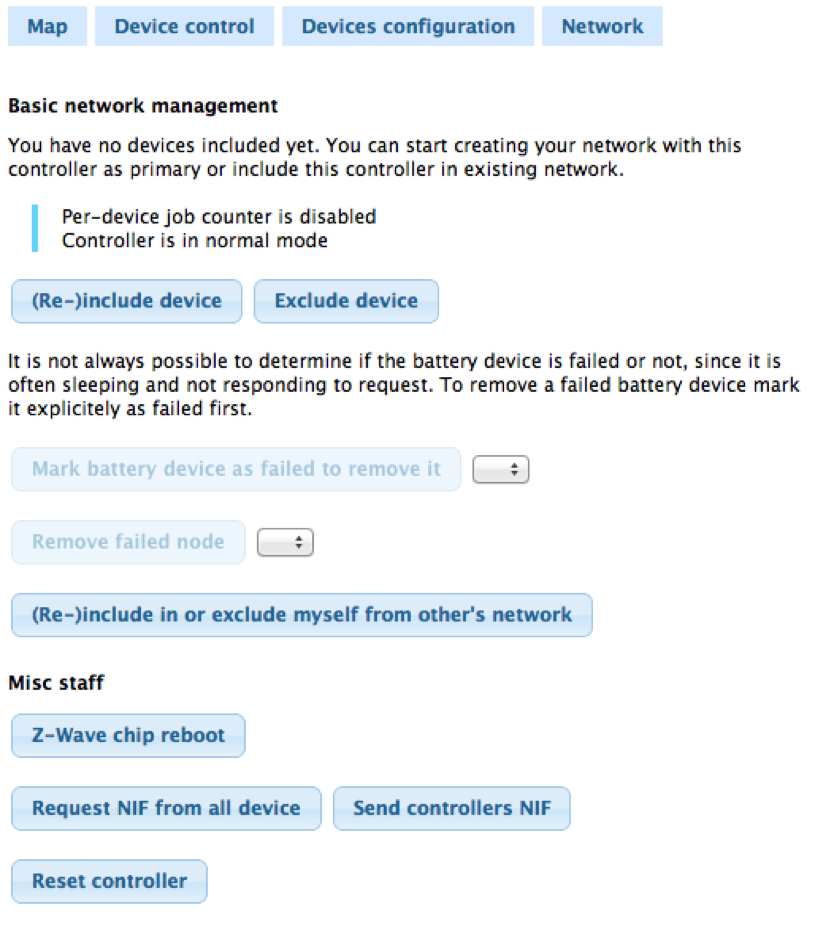
\includegraphics[scale=0.5]{pics/network1.png}
\caption{Network Management}
 
\end{center} 
\end{figure}


The tab 'Network Management' allows including and excluding devices and managing the network. 

\subsection{Inclusion}

You can include devices by pressing the '(Re)Include Device' button. This turns the controller 
into an inclusion mode that allows including a device.  A status information line indicates 
this status. The inclusion of a device is typically confirmed with a triple press of a 
button of this particular device. However, please refer to the manual of this particular 
device for details how to include them into a Z-Wave network. The inclusion mode will time 
out after about 20 seconds or is aborted by pressing the “Stop Include” button.

If the network has a special controller with SIS function \footnote{For more information about
special Z-Wave functions such as SUC or SIS please refer to the book 'Z-Wave Basics'}
(Z-Way will try to activate such 
as function on default, hence this mode should always be active if the USB hardware used by 
Z-Way supports it) the inclusion of further devices can also be accomplished by using the 
include function of any portable remote control which is already included into the network.   
A short explanation above the include button will inform about the ways devices can be included.

\subsection{Exclusion}

You can exclude devices by pressing the 'Exclude Device' button. This turns the controller 
into an exclusion mode that allows excluding a device. The exclusion of a device is typically 
confirmed with a triple press of a button of this particular device as well. However, please 
refer to the manual of this device for details how to exclude them into a Z-Wave network. The 
exclusion mode will time out after about 20 seconds or is aborted by pressing the 
'Stop Include' button.
It is possible to exclude all kind of devices regardless if they were included in the particular 
network of the excluding controller.

If a node is not longer in operation it can not be excluded from the network since exclusion 
needs some confirmation from the device. Please use the 'Remove Failed Node' function in this case. 
Please make sure that only failed nodes are moved this way. Removed but still function nodes 
(called phantom nodes) will harm the network stability.


\subsection{Mark Battery powered devices as failed}

This function allows marking battery-powered devices as failed. Only devices marked as failed can 
be excluded from the network without using the exclusion function. Typically multiple failed 
communications with a device result in this marking. Battery powered devices are recognized as 
sleeping in the controller and therefore all communication attempts with this device will be 
queued until a wakeup notification from this device is received. A faulty battery operated device 
will never send a wakeup notification and hence there is never a communication, which would result 
in a failed node status. Battery operated devices can therefore be manually marked as faulty.  
Make sure to only mark (and subsequently remove) devices that are faulty or have disappeared. 
A device, which was removed with this operation but is still functioning may create malfunctions 
in the network.

\subsection{Remove Failed Nodes}

This function allows you to remove nodes, which are not longer responding or which are not 
available. Please refer to the manual section „Network stability” for further information about 
why failed nodes should be removed.

Z-Way allows removing a node, if and only if this node was detected as failed by the Z-Wave 
transceiver. The network will recognize that communication with a device fails multiple times 
and the device can not be reached using alternating routes either. The controller will then mark 
the device as “failed” but will keep it in the current network configuration.  Any successful 
communication with the device will remove the failed mark. Only devices marked as failed can 
be removed using the 'Remove Failed Node' function.

If you want to remove a node that is in operation use the “Exclude” Function.

\subsection{Include or Exclude myself from other's  network}

Z-Way can join a Z-Wave network as secondary controller. It will change its own Home ID to the 
Home ID of the new network and it will learn all network information from the including controller 
of the new network. To join a different network, the primary controller of this new network needs 
to be in the inclusion mode.

Z-Way needs to be turned into the learn mode using the button “Start Include in others network”. 
The button “Stop Include in others network” can be used to turn off the Learn mode, which will 
time out otherwise or will stop if the learning was successful.

Please be aware that all existing relationships to existing nodes will get lost when the Z-Way 
controller joins a different network. Hence it is recommended to join a different network only 
after a reset with no other nodes already included.


\subsection{Backup and Restore}

The backup and restore function allows to make a backup of the whole configuration of Z-Way 
into a file. The backup will include all included nodes with all their values, status and 
configurations as well as all rules, scenes and timer.

The restore function will overwrite all node values and configuration and automation settings. 
By setting a checkbox the restore function will also overwrite the network topology information 
stored in the Z-Wave chip itself. This will change the home Id of the controller to the home ID 
stored in the backup file. This means that the new controller is an identical clone of the controller 
where the backup is from.

This function needs to be handled with extreme care. Running two identical controllers in one 
network will certainly screw up the settings of both controllers if not doing any further harm. 
Make sure that there is always only one copy of cloned controllers active.

The backup and restore function can be used to move the network between different implementations 
of Z-Way.

\subsection{Z-Wave chip reboot}

This function will perform a soft restart of the firmware of the Z-Wave controller chip without 
deleting any network information or setting. It may be necessary to recover the chip from a 
freezing state. A typical situation of a required chip reboot is if the Z-Wave chip fails to 
come back from the inclusion or exclusion state.

\subsection{Request NIF from all devices}

This function will call the Node Information Frame from all devices in the network. This may be 
needed in case of a hardware change or when all devices where included with a portable USB stick 
such as Aeon Labs Z-Stick.  Mains powered devices will return their NIF immediately, battery operated 
devices will respond after the next wakeup.

\subsection{Send controllers NIF}

In certain network configurations it may be required to send out the Node Information Frame of 
the Z-Way controller. This is particularly useful for the use of some remote controls for 
scene activation. The manual of the remote control will refer to this requirement and give further 
information when and how to use this function.

\subsection{Reset Controller}

The network configuration (assigned node IDs and the routing table and some other network 
management specific parameters) is stored in the Z-Wave transceiver chip and will therefore 
even survive a complete reinstallation of the Z-Way software.

The function “Reset Controller” erases all values stored in the Z-Wave chip and sends the chip 
back to factory defaults. This means that all network information will be lost without recovery option.

This function may create problems if there are still devices included in the network, which 
are not reset to factory default (excluded) before the controller is reset. These devices may 
continue to communicate with the controller regardless if their Node IDs are stored in the 
controller after reset. This can cause all kind of problems. Hence, please handle this 
function with extreme caution!  
Z-Wave-ME hardware does not have this problem anymore!

\subsection{Change Controller - Experts Mode only}

The controller change function allows to handover the primary function to a different controller 
in the network. The function works like a normal inclusion function but will hand over the primary 
privilege to the new controller after inclusion. Z-Way will become a secondary controller of the 
network.
This function may be needed during installation of larger networks based on remote controls only 
where Z-Way is solely used to do a convenient network setup and the primary function is finally 
handed over to one of the remote controls.

\subsection{SUC/SIS Management – Experts Mode only}

This interface allows controlling the SUC/SIS function for the Z-Wave network.

Z-Way will – according to the Z-Wave guideline –always try to become SUC/SIS of a Z-Wave network. 
If Z-Way will remain in the network there is no reason to change the default settings of SUC/SIS.  
In case Z-Way is used as installation controller only it is recommended to turn off the SUC/SIS 
function and assign the SUC/SIS role to a different static controller within the Z-Wave network.


\section{Device Configuration}  

Each Z-Wave device is designed to work out of the box after inclusion without further configuration. 
However it may be suitable and in certain contexts even required doing device specific configurations.

\begin{figure} 
\begin{center}
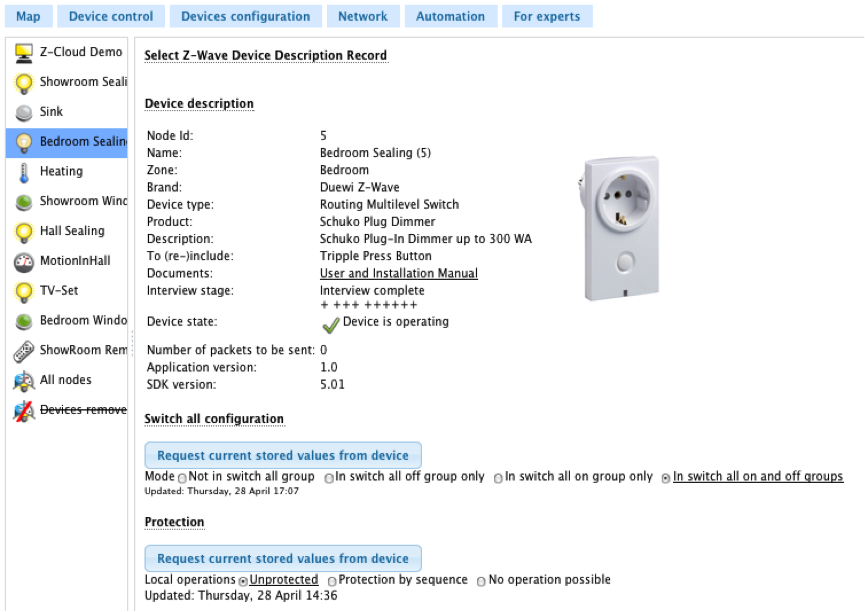
\includegraphics[scale=0.8]{pics/dconfig.png}
\caption{Device Configuration}
\end{center} 
\end{figure} 

The device configuration page allows to further configure the device and to access certain additional 
information about the device. The tab is grouped into several sections. The sections can be toggled 
from invisible to visible and back by clicking on the headlines:

\begin{itemize}
\item  Select Z-Wave Device Description Record
\item  Device Description
\item  Configurations
\item  Actions with configurations
\item  Advanced Actions
\end{itemize}


\subsection{Interview Process}
After the inclusion of a new device Z-Way will interview the device just included. The interview is a 
series of commands Z-Way is sending to the device in order to learn the capabilities and functions 
of this device.
Depending on the capabilities announced in the Node Information Frame that was received during 
the „Device Status“ tab will indicate if the interview was successfully completed.  The blue 
information icon shows if the interview was not complete. Clicking on this icon opens a dialog with 
all command classes and the status of their respective interviews.  
A complete interview is important in order to have access to all functions of the device included. 
Incomplete interviews may also be a reason for malfunctions of the network.
There are several reasons why an interview may not be completed.
\begin{enumerate}
\item  A battery-operated device may be gone into sleep mode too early. In this case is possible to 
wake up the device manually to complete the interview. Sometimes manual wakeup is needed several times.
\item  The device does not fully comply with the Z-Wave protocol. This is particularly possible for 
devices that were brought to market before 2008. The current more sophisticated certification 
process makes sure that devices are 100\% compatible to the Z-Wave product when they hit the market.   
Please check online information (wiki, forums) on details and possible ways to fix these kinds of problems.
\item  The device does not have a reliable communication route to the controller. Interview 
communication typically use longer packets than normal polling communication. This makes the 
interview communication more vulnerable against weak and instable communication links. It is 
possible that the controller is able to include a device and even receive confirmation of a 
polling request but still not being able to complete the interview. However this is a rare case.
\item  The device may be simply broken.
\end{enumerate}

\subsection{Select Z-Wave Device Description Record}

After a successful inclusion Z-Way will interview the device to gather further information.  

\subsubsection{Select Device Description Record}

Certain information such as names of association group, the brand name of the device and the parameters 
of further configuration values can not be detected during interview. Z-Way uses a device database with 
product description files to obtain this information. In order to identify the right device description 
record certain parameters of the interview are used. 
If these parameters match exactly one device description record this very record is loaded and its 
content is shown on the device configuration page automatically.

If the information from the device is sufficient to select one specific record from the database this 
section of the tab is hidden. If it is not possible to identify the correct device description record 
the user can manually choose the correct record. It is also possible to manually change the selection 
of the device description by unhiding this section and clicking on the “Select Device Description 
Record” button.

\subsubsection{Request NIF}  

This function requests the selected device to send its Node Information frame (NIF) to the controller. It 
can be used instead of triple pressing a button on the device itself that would also instruct the device 
to send its NIF. The NIF is needed to know device capabilities.


\subsection{Device Description}

The upper part of the dialog shows some descriptive values of the device.  The Z-Wave device type 
is the only value generated solely from the interview data. All other data are taken from the device 
description record.
\begin{itemize}
\item  {\bf Zone:} This is the zone/room the device is assigned to. Will be manually defined in Zone-tab.

\item  {\bf Brand:} This is the product code or brand name of the device. This will be taken from the device description record.

\item  {\bf Device Type:} This is the type of Z-Wave device as reported by the device during inclusion.

\item  {\bf Description:} This is a verbal description of the function. This will be taken from the device description record.

\item  {\bf Interview Stage:} This shows the progress of the interview process. This information is generated by Z-Way.

\item  {\bf Inclusion Note:} How to (re-) include the device. This will be taken from the device description record.

\item  {\bf Wakeup Note:} This will be taken from the device description record.

\item  {\bf Documents:} If the device description record offers links to manuals or other online documents there are 
shown here. This will be taken from the device description record.

\item  {\bf Device State:}  Status of the device plus number of packets queued for this device
\end{itemize}
 
There are a couple of reasons why no device description record was found:
\begin{itemize}
\item  There is no record for the device available. Since there are always new devices on the 
market, Z-Way needs to catch up and update its device database. If your device is not found, 
updating to the most recent version of Z-Way may help.
\item  The interview was not finished to the point where enough parameters were detected to identify 
the correct device description record. You may manually choose the correct device description record 
using the button “Select Device Description Record”. A dialog box will be opened for manual selection 
of the product (if available). The manual selection of a device description record is only needed if 
no record was found on default.  
\item  The interview of the device was completed but the device does not offer enough information to 
identify the correct device. You may manually choose the correct device description record using the 
button “Select Device Description Record”. A dialog box will be opened for manual selection of the 
product (if available). The manual selection of a device description record is only needed if no 
record was found on default.
\item  There is more than one device description record matching the information gathered during 
interview.  This is particularly possible if a vendor sells devices with different firmware and 
functions without properly updating the firmware version information. You may manually choose the 
correct device description record using the button “Select Device Description Record”. A dialog box 
will be opened for manual selection of the product (if available). The manual selection of a device 
description record is only needed if no record was found on default.
\end{itemize}
\subsection{Associations}

To interconnect the different sources of switching events (sensors, remote controls, wall controllers) 
with real switches (power switches, dimmers, window blinds, thermostats) Z-Wave introduces the concept 
of Association.

An Association is a relationship between a sensor or controller and an actor with the result that 
any events triggered by the sensor or manually activated by a button on the controller results in 
sending a switching command to an actor or a group of actors.

\quote{Examples:}

In order to switch a simple power switch with a remote control, this certain button of a remote control 
needs to be associated to the power switch.

In order to close the window blind during darkness the luminescence sensor issuing a command when the 
light level changes below a certain level or raises above a certain level needs to be associated 
with a window blind. 

Z-Wave devices supporting association (means supporting to control other devices) offer a number 
of so called association groups.  Each group refers to a single event within the device, which may 
cause sending out commands to other Z-Wave device. The user can assign certain actors to these 
groups and all members of these groups will receive a switching command if this group gets activated. 
Typically these groups are referred to a button (association group Button 1) or a special event of
a device (association group for battery status messages or association group for triggering a door sensor)

The command used for associations is typically a simple “SET to Value X” with X as a definable value. 
This certainly limits the flexibility of associations but allows a simple and fast setup of
interrelations between sensors, controllers and actors.
 
If there was no previous device of the same type installed the interface will show the values as 
read from the device. If there was already a device of the same kind installed there may exist a 
stored default configuration for this particular device. Then the setup in the device may differ 
from the default configuration stored in Z-Way.

\begin{itemize}
\item  Gray Icon: This Node ID is stored in the device but its not stored in the default configuration 
of the Z-Way. You can double click this device to store this setting in the Z-Way default configuration 
of this device type.

\item  Red Icon: This Node ID is stored locally but not in the association group of the device yet. 
Apply the settings to transmit the setting into the device.  In case of a battery operated device you 
need to wakeup the device in order to store the configuration.

\item  Black Icon: This Node ID is stored both in the device and in the local configuration of Z-Way.
\end{itemize}
Hint: The auto configuration function of Z-Way will place the node ID of the Z-Way controller in all 
association groups if possible. This allows the activation of scenes from these devices. 

\subsection{Configurations}

If a Device Description Record was loaded this section will show device specific configuration values 
including their possible parameters and a short description of the configuration value. You may change 
these values according to your needs.

The most important action in regard to the configuration is to apply the configuration to the device. 
This is only done when the button “Apply configuration for this device” is hit. This button is 
therefore even shown, when the rest of the tab part is hidden.
\begin{itemize}
\item  Mains Powered Devices: The settings will become effective immediately after hitting the button.
\item  Battery Powered Devices: The settings will become effective after the next wakeup of the device, 
as shown in the Device Status tab.
\item  Battery Powered Controllers (remote controls or wall controllers): The settings will only become 
effective if the devices are woken up manually. Refer to the controller manual for more information 
on how to wake up the device. 
\end{itemize}

\subsection{Actions with Configurations}

If there are many similar devices in a network it is desirable to just apply one working configuration 
to all these devices. This can be done using the function 'Copy from other Device'.

The set of defined configuration values is stored for every device. Therefore its possible to pick a 
different device and reuse its configuration values for the device to be configured.  The 'Save' 
function of the bottom context menu allows saving the configuration for further use and reuse.

\subsection{Advanced Actions - Expert Mode only}

\subsubsection{Force Interview}  

This functions forces to redo the whole interview. All previous interview data will be deleted. This 
function is for debugging purposes only.

\subsubsection{Show Interview Results} 
This function shows the result of the interview. This function is for debugging purposes only. For 
information about reasons for incomplete interview please refer to the manual section “Device Status”.

\subsubsection{Switch to raw mode}

This function turns the configuration dialog into a generic mode. 

The bottom context menu function  „Reset Configuration“ deletes all configurations stored in Z-Way, 
but does not affect devices!

\section{Device Operation}

This section describes interface tabs to access functions of the Z-Wave devices.

\subsection{Switches}

\begin{figure} 
\begin{center}
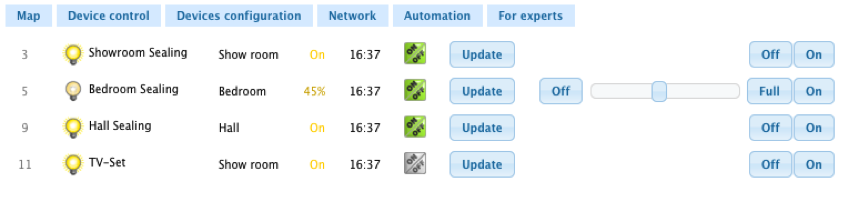
\includegraphics[scale=0.8]{pics/switches.png}
\caption{Switches}
\end{center} 
\end{figure} 

This page gives a table style overview of all actuators of the Z-Wave network. Actuators are devices 
with some kind of switching function such as 
\begin{itemize}
\item Digital (on/off) switches, 
\item Light Dimmer, 
\item Motor Controls for Venetian blinds, window bind,
\item Motor Control to open/close doors and windows.
\end{itemize}

Beside the name of the device, the location and the type of the device, the actual status and the 
timestamp of this status are shown.

Of course it is possible to switch the devices and to update the status of the device.

A little icon indicates how the device will react to a “switch all devices” command  
(will switch, will not switch, will react to off command only or to on command only).

\subsection{Sensors} 


\begin{figure} 
\begin{center}
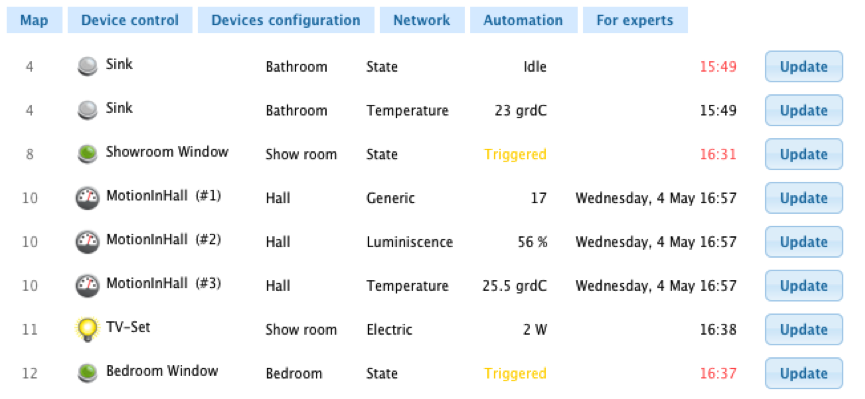
\includegraphics[scale=0.7]{pics/sensors.png}
\caption{Sensors}
\end{center} 
\end{figure}

This page gives a table style overview of all sensors of the Z-Wave network.  
Sensors are devices able to report measured values. Sensors can report binary or analog values.  
Beside the name of the device, the location and the type of sensor the actual sensor value and 
the timestamp of this value are shown. It is possible to ask for an update of the sensor value.

\subsection{Meter Overview}

This page gives a table style overview of all meters of the Z-Wave network.  
Meters are devices able to report accumulated values.  Beside the name of the device, the location 
and the type of meter, the actual meter value and the timestamp of this value are shown. 
It is possible to ask for an update of the meter value.

\subsection{Thermostats}

Z-Way allows setting the desired temperature of the thermostat and access the setpoint.

\subsection{Locks}

This section allows operating door locks.

\section{Maintenance}

\subsection{Device Status overview}

\begin{figure} 
\begin{center}
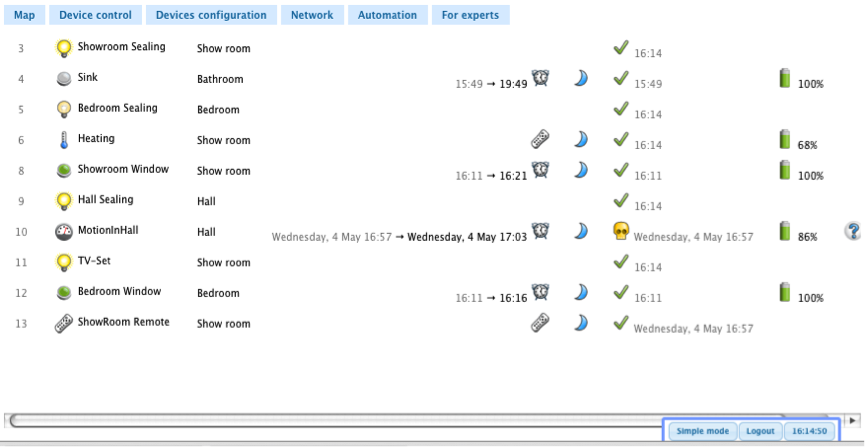
\includegraphics[scale=0.7]{pics/devicestatus.png}
\caption{Device Status Overview}
\end{center} 
\end{figure}

This tab gives an overview of the network status and the availability of each device. It shows the 
timestamp of the last interaction between the controller and the device. For battery powered devices the 
battery charging status, the time of the last wakeup and the estimated time for the next wakeup is shown.
An info icon indicates when the interview of a device was not completed. Clicking on this device opens 
a window showing the interface status by command class. Please refer to the manual section “Interview” 
for more information about the interview process.

\subsection{Routing}

\begin{figure} 
\begin{center}
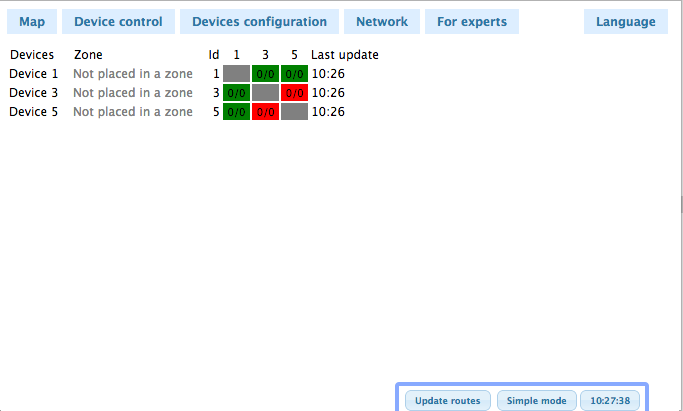
\includegraphics[scale=0.5]{pics/routingtable.png}
\caption{Routing Table}
\end{center} 
\end{figure}
The routing table of the Z-Wave network is shown as second submenu of the network tab. It indicates how 
two devices of the Z-Wave network can 
communicate with each other. If two devices are in direct range (they can communicate without the help of 
any other node) the cross point of the two devices in the table is marked as dark green. The color 
light green indicates that the two nodes are not in direct range but have more than one alternating 
routes with one node between. This is still considered as a stable connection.
The yellow color indicates that there are less than two “one-hop” routes available between the two 
nodes. However there may be more routes but with more nodes between and therefore considered as less stable.

A red indicator shows that there are no good short connections between the two nodes. This does not 
mean that they are unable to communicate with each other but any route with more than 2 routers 
between Z-Way is considered as not reliable, even taking into account that Z-Wave supports routes 
with up to four devices between. Grey cells indicate the connection to the own Node ID. 


\begin{quote} {\bf The general rule of thumb is: “The greener the better”} 
\end{quote}

The table lists all nodes on the y-axis and the neighborhood information on the x-axis. On the 
right hand side of the table a timestamp shows when the neighborhood information for a given node 
was reported.   

In theory the table should be totally symmetric, however different times of the neighborhood detection 
may result in different neighborhood information of the two devices involved.
 
The neighbor information of the controller works with an exception. The Z-Wave implementation used 
in current Z-Wave transceiver does not allow requesting an update of the neighbor list for the 
controller itself. The neighborhood information displayed for the controllers therefore simply wrong.

Battery powered devices will report their neighbors when woken up and report their mains powered 
neighbor correctly. However mains powered devices will report battery-powered devices as neighbors 
only when routes are updated twice. This is less critical because battery powered devices can not be 
used as routers and are therefore not relevant for calculating the route between two nodes anyway. 
 
The context menu command “Network Reorganization” allows re-detecting all neighborhood 
information (battery powered devices will report after their next wakeup!)  

\section{Debugging / Expert Mode}

The „Expert Mode“ button in the bottom context menu switches between a standard mode and expert mode. 
In expert mode some more technically oriented dialogs are available. A detailed description
of these dialogs can be found in the Z-Way Developers Documentation.

  
\end{document} 
